\chapter{XSD}

Dans cette partie, nous expliquerons notre conception de la partie validation d'un document XML à partir d'un document XSD.

\section{Hypothèses simplificatrices}
	Afin de simplifier l'implémentation du parseur XSD, les hypothèses suivantes ont été posées :
	\begin{itemize}
		\item{Les types simples seront de type \textit{string} ou \textit{date}}
		\item{Les types complexes seront de type \textit{sequence} ou \textit{choice} et pourront contenir des attributs}
	\end{itemize}

\section{Fonctionalités implémentées}
Les points suivants sont pris en charge par le validateur XSD :
\begin{itemize}
    \item{Choix d'éléments racine multiples}
    \item{Présence et type des attributs}
    \item{Éléments de types \textit{mixed}}
    \item{Types complexes contenant des éléments \textit{sequence} et \textit{choice} imbriqués}
    \item{Nombre d'occurences minimum et maximum par élément}
    \item{Références sur des attributs, éléments et types}
\end{itemize}

\section{Diagramme de classes}
Les classes ici décrites seront rattachées au \textit{\lstinline$namespace Xsd$} défini en C++.

\begin{landscape}
\begin{figure}[H]
	\centering
	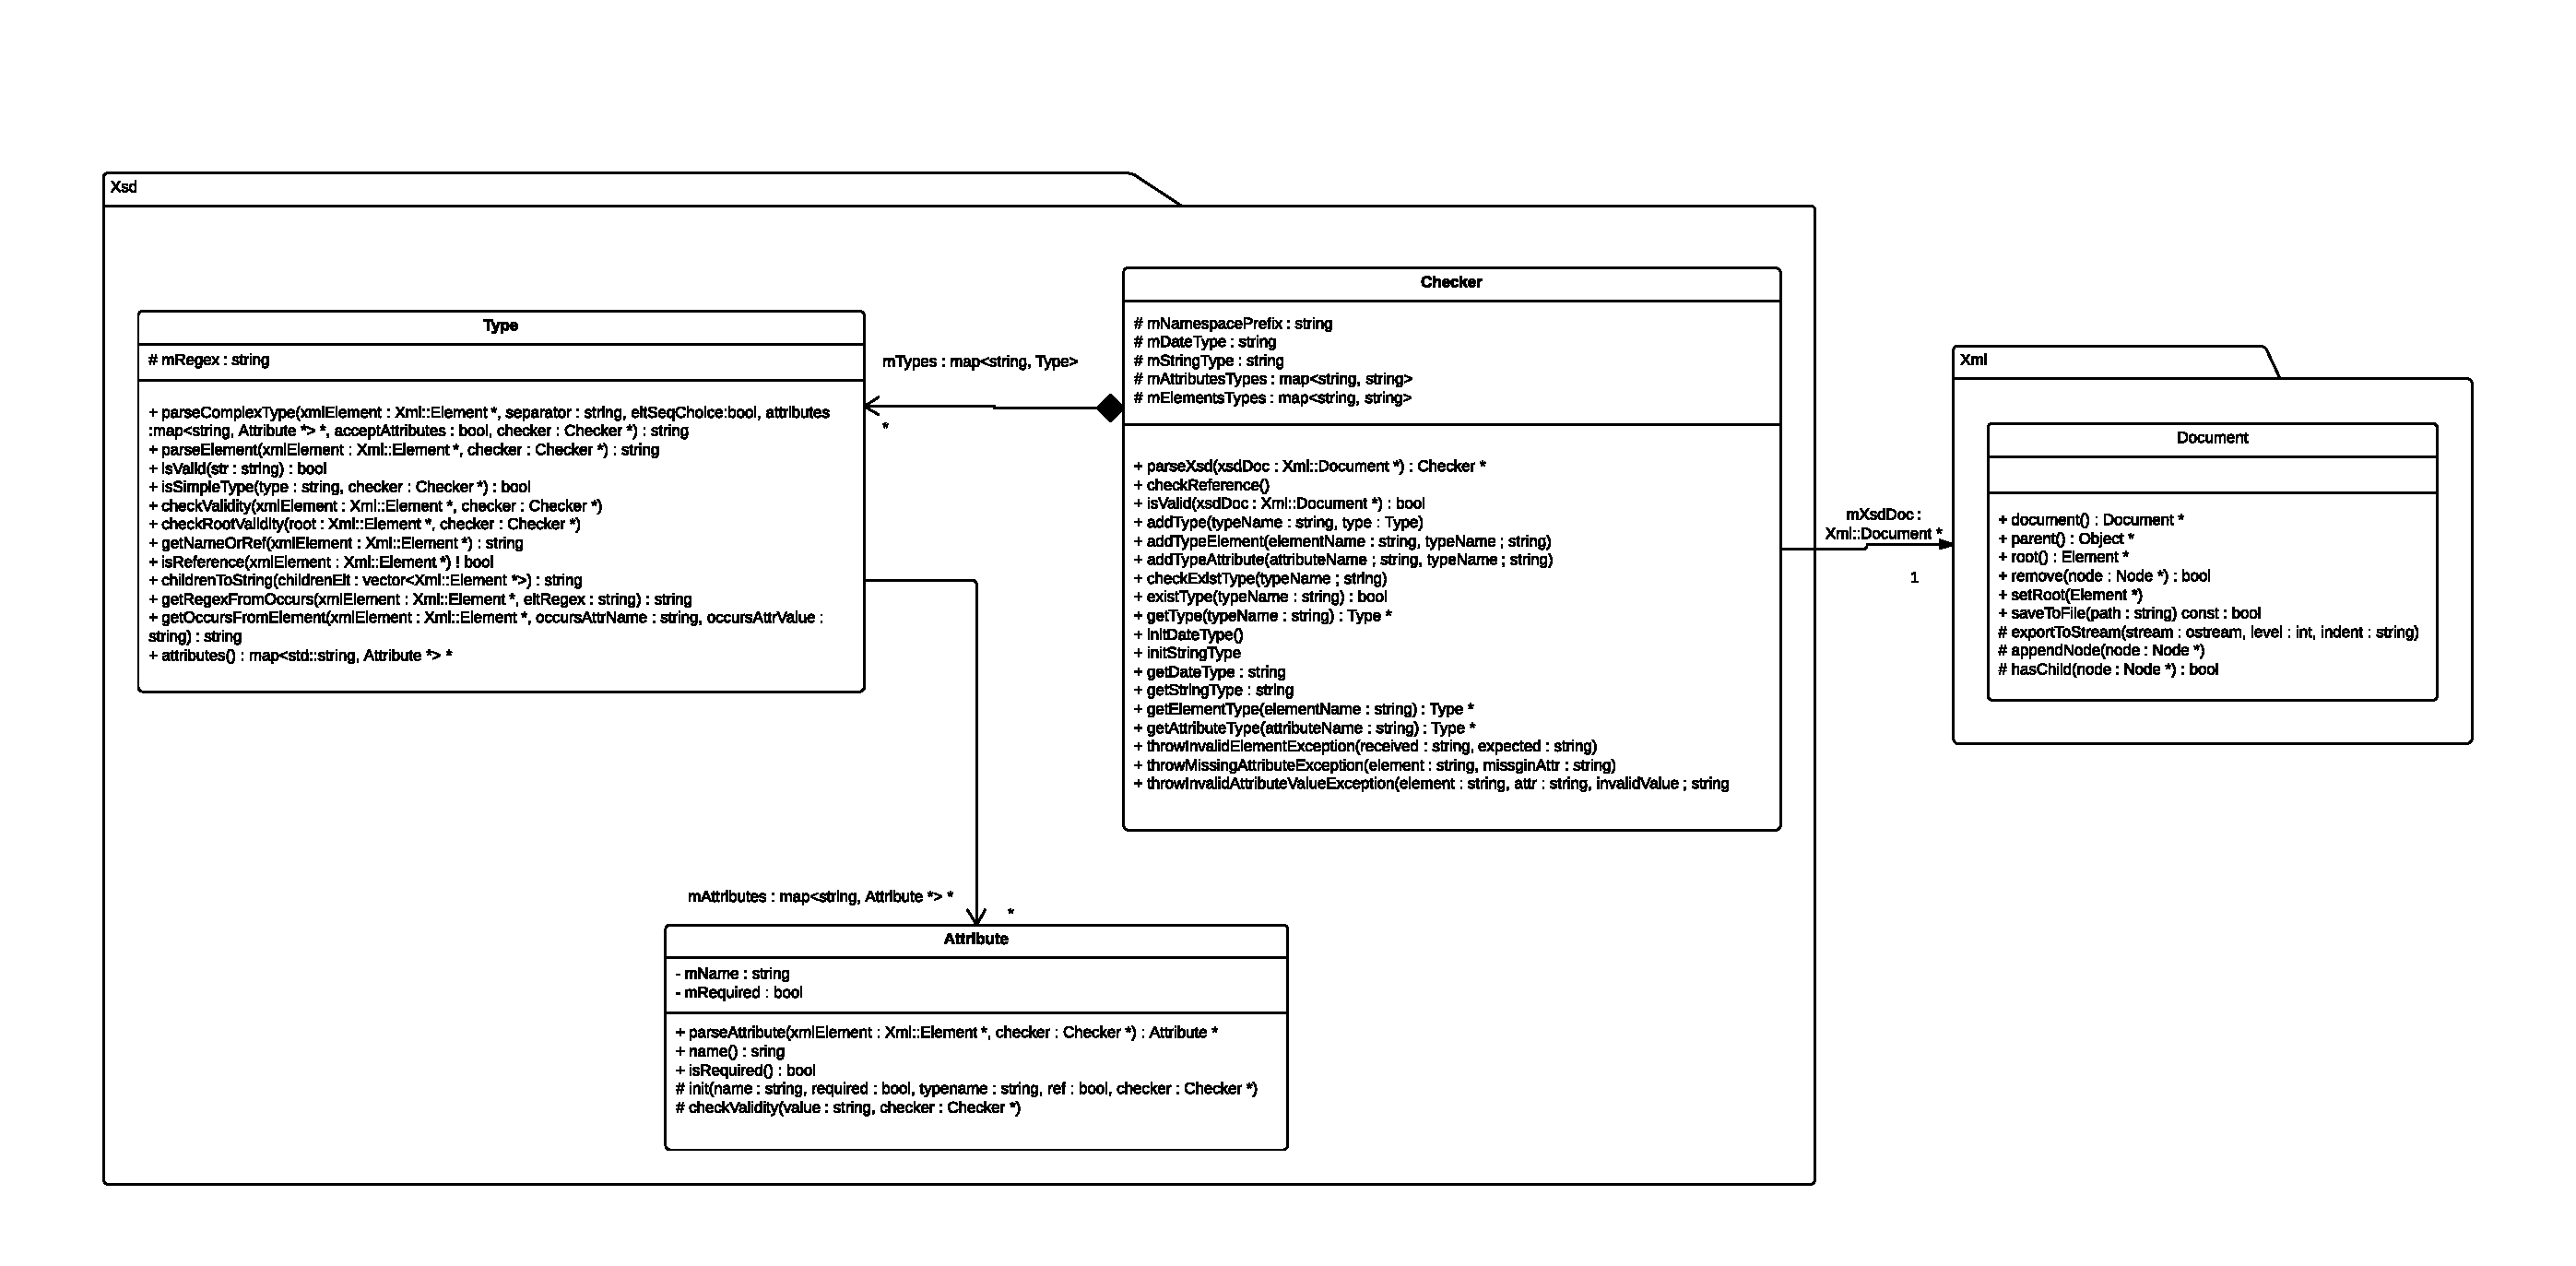
\includegraphics[width=1\linewidth]{images/xsd-uml.pdf}
	\caption{Diagramme de classe de la validation xsd}
	\label{xsdClassDiagram}
\end{figure}
\end{landscape}

\section{Entités}
	\subsection{Checker}
		Un objet Checker décrit les règles présentes dans un document XSD. Les méthodes principales sont les suivantes :
		\begin{itemize}
			\item \textbf{parseXsd} : méthode statique retournant un objet de type \textit{Checker},  construit à partir du document XSD passé en paramètre
			\item \textbf{isValid} : retourne \textit{true} si le document XML passé en paramètre est en accord avec les contraintes inscrites dans l'objet \textit{Checker} courant, \textit{false} sinon
		\end{itemize}

		La structure intermédiaire s'appuie sur 3 tables de hachages :
		\begin{itemize}
			\item \textbf{mTypes} : associe le nom (chaîne de caractères) d'un type avec son objet de type \textit{Type}
			\item \textbf{mElementsTypes} : associe le nom d'un élément avec le nom de son type
			\item \textbf{mAttributesTypes} : associe le nom d'un attribut avec le nom de son type
		\end{itemize}

	\subsection{Element}
		Un élément est une chaîne de caractères, associé\footnote{Dans la suite de cette partie, le terme \textit{associer} correspondra à l'insertion d'une paire clé/valeur dans une table de hachage} à un type dans la table de hachage \textit{mElementsTypes} d'un objet de type \textit{Checker}.

	\subsection{Type}
		On objet \textit{Type} correspond à un type complexe XSD. Il est défini par deux éléments :
		\textit{Expression régulière} : Cette chaîne de caractères détermine l'ensemble des fils directs que l'élément rattaché au type peut recevoir. Elle spécifie leur ordre et nombre d'occurences.
			\textbf{Exemple} : \textit{(<fromage>){4}|(<poisson>){1})} sera l'expression régulière du type associé à l'élément \textit{pizza}.
			Elle indique qu'une pizza peut contenir 4 fromages ou un poisson.
		\textit{Liste d'attributs} : Cette liste décrit les attributs que contiendra l'élément rattaché au type courant, l'ordre des attributs n'ayant pas d'importance.

	\subsection{Attribute}
		Un attribut est décrit par son nom et un attribut \textit{required} à \textit{true} ou \textit{false}. Il est également associé à un type dans la table de hachage \textit{mAttributesTypes}.

\section{Algorithme}

\subsection{Construction de la structure intermédiaire}
L'algorithme présent construit un objet Checker, lequel contiendra un ensemble de types et attributs.
Cet algorithme parcours en une passe l'arbre XML obtenu lors du parsing préalable du document XSD.
Il s'agît d'un algorithme récursif, le parcours de l'arbre XML pouvant être assimilé à un parseur de type SAX sur le document XSD.

	\subsubsection{Parsing du document XSD : \textit{parseXsd}}
		\lstinline$Parsing du document XSD sous forme d arbre XML$\\
		\lstinline$Parsing du type de l element racine (c.f. parseComplexType)$\\ \footnote{L élément \textit{schema} est implicitement de type complexe, ses éléments fils sont traités comme s ils étaient dans un élément \textit{choice}}
		\lstinline$Association du "ROOT_TYPE" avec le type recu$\\
		\lstinline$Association du nom d element "ROOT" avec le type recu$\\
		\lstinline$Verification des references (c.f. checkReferences)$\\

	\subsubsection{Parsing d'un élément \textit{complexType} : \textit{parseComplexType}}
		\lstinline$SI l element complexType a un attribut mixed a true$\\
		\indent \lstinline$Ajout de ".*" au separateur d elements de la regex$\\

		\lstinline$Parcours des fils de l element complextype$\\
		\indent \lstinline$SI c est un element sequence$\\
		\indent \indent \lstinline$Appel recursif$\\
		\indent \lstinline$SI c est un element choice$\\
		\indent \indent \lstinline$Appel recursif avec le separateur "|"$\\
		\indent \lstinline$SI c est un element element$\\
		\indent \indent \lstinline$on ajoute a la regex de l element complexType celle de l element retournee par parseElement() + le separateur$\\
		\indent \lstinline$SI c est un element attribute$\\
		\indent \indent \lstinline$Parsing de l attribut (c.f. parseAttribute)$\\
		\indent \indent \lstinline$Ajout de l attribut a la map d attributs du type courant$\\

		\lstinline$On retourne la regex associee au type$\\


	\subsubsection{Parsing d'un élément \textit{element} XSD : \textit{parseElement}}
		\lstinline$Construction d une regex decrivant l element en fonction de ses occurences$\\ \footnote{Par exemple, pour <xsd:element name="parfum" type="xsd:string" minOccurs="1" maxOccurs="2"/> on generera l expression (<pizza>){1}((<pizza>)?){1}}
		\lstinline$SI ce n est pas une reference$\\
		\indent \lstinline$SI l element a des enfants (c est un type complexe)$\\
		\indent \indent \lstinline$Construction d un type avec le premier fils de l element$\\ \footnote{Le constructeur de type appelle \textit{parseComplexType}}
		\indent \indent \lstinline$Association du nom du type avec le type construit$\\
		\indent \lstinline$Association du nom de l element avec le nom du type construit$\\
		\lstinline$On retourne la regex associee a l element$\\


	\subsubsection{Parsing d'un élément \textit{attribute} : \textit{parseAttribute}}
		\lstinline$SI les attributs nom et type sont definis, et que c est un type simple$\\
		\indent \lstinline$Association du nom de l attribut avec le nom du type$\\
		\lstinline$On retourne un nouvel attribut a partir d un nom et d un booleen required$\\


	\subsubsection{Vérification des références : \textit{checkReferences}}
		\lstinline$Pour chaque element$\\
		\indent \lstinline$On verifie que l element est rattache a un type dans mElementsTypes$\\
		\lstinline$Pour chaque type$\\
		\indent \lstinline$Pour chaque attribut du type$\\
		\indent \indent \lstinline$On verifie que l attribut est rattache a un type dans mAttributesTypes$\\

\pagebreak

\subsection{Validation d'un document XML}
	\subsubsection{Validation d'un type : \textit{checkValidity}}
		Cette méthode prend un élément XML en paramètre, et valide les attributs qu'il contient et l'architecture de ses fils directs.
		L'appel initial est donc fait sur le type associé au nom de l élément root XML

		\lstinline$On verifie que l ensemble des attributs de l element XML existent dans la map des attributs du type XSD$\\
		\lstinline$Pour chaque attribut XSD du type XSD$\\
		\indent \lstinline$Si l attribut XSD existe$\\
		\indent \indent \lstinline$On verifie que sa valeur valide l expression reguliere de son type$\\
		\indent \lstinline$Si l attribut XSD n existe pas$\\
		\indent \indent \lstinline$On verifie qu il n est pas requis$\\

		\lstinline$Generation d une chaine de caracteres correspondant a la concatenation des balises de ses elements fils$\\
		\lstinline$On verifie que l expression reguliere du type valide cette chaine de caracteres$\\

		\lstinline$Pour chaque element fils de l element XML recu$\\
		\indent \lstinline$Recuperation du type associe au nom du fils$\\
		\indent \lstinline$Appel recursif a la fonction checkValidity sur le type obtenu$\\

